% \iffalse meta-comment
%<=*COPYRIGHT>
%% Copyright (C) 2012 by Martin Scharrer <martin@scharrer-online.de>
%% -----------------------------------------------------------------------
%% This work may be distributed and/or modified under the
%% conditions of the LaTeX Project Public License, either version 1.3
%% of this license or (at your option) any later version.
%% The latest version of this license is in
%%   http://www.latex-project.org/lppl.txt
%% and version 1.3 or later is part of all distributions of LaTeX
%% version 2005/12/01 or later.
%%
%% This work has the LPPL maintenance status `maintained'.
%%
%% The Current Maintainer of this work is Martin Scharrer.
%%
%% This work consists of the files mwe.dtx and mwe.ins and multiple
%% example-*.tex files
%% and the derived filebase mwe.sty and example-*.{pdf,eps,png,eps}.
%%
%<=/COPYRIGHT>
% \fi
%
% \iffalse
%<*driver>
\ProvidesFile{mwe.dtx}[%
%<=*DATE>
    2012/05/15
%<=/DATE>
%<=*VERSION>
    v0.3
%<=/VERSION>
    DTX file for mwe]
\documentclass{ydoc}
\GetFileInfo{mwe.dtx}
\usepackage{mwe}[\filedate]
\usepackage[export]{adjustbox}
\usepackage{flafter}
\EnableCrossrefs
\CodelineIndex
\RecordChanges
\OnlyDescription
\begin{document}
  \DocInput{\jobname.dtx}
  \PrintChanges
  \PrintIndex
\end{document}
%</driver>
% \fi
%
% \CheckSum{0}
%
% \CharacterTable
%  {Upper-case    \A\B\C\D\E\F\G\H\I\J\K\L\M\N\O\P\Q\R\S\T\U\V\W\X\Y\Z
%   Lower-case    \a\b\c\d\e\f\g\h\i\j\k\l\m\n\o\p\q\r\s\t\u\v\w\x\y\z
%   Digits        \0\1\2\3\4\5\6\7\8\9
%   Exclamation   \!     Double quote  \"     Hash (number) \#
%   Dollar        \$     Percent       \%     Ampersand     \&
%   Acute accent  \'     Left paren    \(     Right paren   \)
%   Asterisk      \*     Plus          \+     Comma         \,
%   Minus         \-     Point         \.     Solidus       \/
%   Colon         \:     Semicolon     \;     Less than     \<
%   Equals        \=     Greater than  \>     Question mark \?
%   Commercial at \@     Left bracket  \[     Backslash     \\
%   Right bracket \]     Circumflex    \^     Underscore    \_
%   Grave accent  \`     Left brace    \{     Vertical bar  \|
%   Right brace   \}     Tilde         \~}
%
%
% \changes{v0.1}{2012/05/03}{Initial version.}
% \changes{v0.2}{2012/05/08}{Added ``example-'' prefix to image files.}
% \changes{v0.3}{2012/05/15}{Added graphicspath for ``example-'' and moved PDF to the begin of the file extensions.}
%
% \DoNotIndex{\newcommand,\newenvironment}
%
% \GetFileInfo{mwe.dtx}
% \author{Martin Scharrer}
% \email{martin@scharrer-online.de}
% \repository{https://bitbucket.org/martin_scharrer/mwe}
%
% \maketitle
%
% \begin{abstract}\noindent
% The \pkg{mwe} CTAN package comes with a small \LaTeX\ package which loads
% packages commonly used to create minimal working examples (MWEs)
% and with a collection of dummy images. The idea is that this images
% are installed in the \texttt{TEXMF} tree in a way where they are accessible
% by any document. Then MWEs with images can be shared by multiple users
% without the need of image replacement code or the \texttt{dummy} option of \texttt{graphicx}.
% \end{abstract}
%
% \section{Introduction and Motivation}
% \LaTeX\ has a large online-community and people can find a lot of help from other users
% on places like
% \href{https://groups.google.com/forum/?fromgroups#!forum/comp.text.tex}{\texttt{comp.text.tex}}
% or \url{http://tex.stackexchange.com/}.
% In many cases the user with the problem is required to post a code example which shows
% the use-case, but nothing unrelated, and should be compilable by other people without extra effort.
% Such an example is often called a \emph{minimal working example} (MWE), or sometimes only \emph{minimal example}.
% Users can use this example document to test if the issue also occurs in their \LaTeX\ installation and
% easily implement and test solutions. If a solution is found the modified example can be posted back to the original
% user. For general questions like "How to do X", answers often create an example document by themselves.
%
% There are some packages which are very useful for MWEs (and mostly only for these), like the \pkg{lipsum}
% and \pkg{blindtext} packages. Both produce dummy text in the document which is required to produce realistic scenarios
% for e.g.\ float placement etc. This frees the user from typing or copying larger dummy texts by himself,
% which would also increase the size of the example and make it less readable.
% The \pkg{mwe} package loads such packages and allows for a further reduction of the MWE document size.
%
% A problem with sharing MWEs appears if image files are included in the document (e.g.\ \Macro\includegraphics,
% \env{figure} environments etc.). Often the image is replaced with a replacement code like
% \Macro\rule{<width>}{<height>} or the \texttt{demo} option of \pkg{graphicx} is used to replace the image with an
% empty frame without trying to read the given image file.
% Both of these methods are a little cumbersome and have other issues. For once, an explanation for new users must be
% added to replace the code with a real \Macro\includegraphics or to remove the \texttt{demo} option for their final
% document. Another issue might arise when the example requires specific image options like scaling or cropping,
% which might not be easily and completely be replicated with these replacements.
% Also, the compiled result will look less than a normal document with real images.
%
% To overcome these drawbacks several real dummy images with different sizes, ratios and formats are provided with
% this package. Once installed in the correct directory in the \texttt{TEXMF} tree they will be available to all
% documents. This way a user can compile any MWE given to him by another person
% which uses these image files without requiring code replacements or sharing images. The \pkg{mwe}, which loads
% \pkg{graphicx}, can be used to minimise the preamble, but is not required to be loaded in order to use the images.
%
% It should be noted that the main contribution of this CTAN package is, at least at the moment, the provided demo/test image files.
% The \pkg{mwe} \LaTeX\ package is (in his current form) just an addition.
%
% \section{Usage}
% The provided image files can be included as normal using i.e.\ using the \pkg{graphicx} package and its
% \Macro\includegraphics[<options>]{<filename>} macro.
% They are also provided in source code form (\texttt{.tex} files) and can be included in a document
% using \Macro\input{<filename>}. They require the \pkg{tikz} package to be loaded.
% For this to work it is important that the images are located at the indented position in the \texttt{TEXMF} tree as
% described in section~\ref{sec:installation}.
%
% The \pkg{mwe} can be loaded in the preamble of a MWE and loads often used packages.
% At this moment these are only \pkg{graphicx}, \pkg{lipsum} and \pkg{blindtext}, while the last two are only
% loaded if they are installed. The package is not required for using the image files.
% If the package is loaded it will change the graphic extension list so that PDF files are used first for formats which
% support PDF images. Also \Macro\graphicspath{{example-}} is used to allow to shorten the file names to `|image..|'
% instead of the full `|example-image...|'.
%
% Some MWE might even be better off not to use the package if specific side-effect between packages is tested.
%
% \begin{lstlisting}[language={[latex]tex},gobble=4,title={Usage Example}]
%   \documentclass{article}
%   \usepackage{mwe}% or load 'graphicx' and 'blindtext' manually
%   \begin{document}
%   \blindtext
%   \begin{figure}
%   
\includegraphics[width=.48\linewidth]{example-image-a}\hfill
%   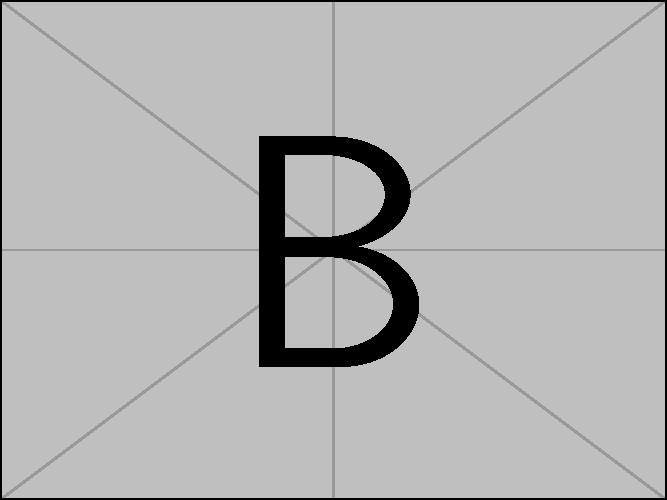
\includegraphics[width=.48\linewidth]{example-image-b}
%   \caption{MWE to demonstrate how to place to images side-by-side}
%   \end{figure}
%   \blindtext
%   \end{document}
% \end{lstlisting}
%
%
%
% \section{Installation}\label{sec:installation}
% The \pkg{mwe} package has due to its nature a little uncommon installation requirements.
% While the normal package files are installed as normal, a variety of image files
% are installed in the \texttt{tex/latex/mwe/} folder, so that they can be accessed from
% every (MWE) document.
%
% Multiple binary images are included which can't be build from the DTX alone
% without extra conversion tools.  A TDS ZIP file which only needs to be unzipped
% over the TEXMF is also provided.  This is the preferred way to install this
% package for end users and distribution maintainers.  If a manual build is wanted
% change all occurrences of `|nostandalone|' to `|standalone|' in the DTX file.
% Compile all extracted TEX files with |pdflatex| and convert these files from PDF
% to PNG and JPG. Compile again with |latex| and |dvips| to create the EPS files
% (rename the PS to EPS).
%
% \begin{center}
% \begin{tabular}{>{\ttfamily}l>{\ttfamily}l}
%   \toprule
%    \normalfont  Files & \normalfont\hskip-3em TEXMF Installation folder \\
%   \midrule
%     mwe.dtx mwe.ins                                 & source/latex/mwe/ \\
%     mwe.pdf README INSTALL                          & doc/latex/mwe/    \\
%     mwe.sty                                         & tex/latex/mwe/    \\
%     example-image-*x*.\{tex,pdf,png,jpg,eps\}       & tex/latex/mwe/    \\
%     example-image-?.\{tex,pdf,png,jpg,eps\}         & tex/latex/mwe/    \\
%     example-image-golden*.\{tex,pdf,png,jpg,eps\}   & tex/latex/mwe/    \\
%     example-grid-*.{tex,pdf}                        & tex/latex/mwe/    \\
%     example-image-a?*.pdf example-image-letter*.pdf & tex/latex/mwe/    \\
%     example-image-a?*.tex example-image-letter*.tex & source/latex/mwe/ \\
%   \bottomrule
% \end{tabular}
% \end{center}
%
%
% \section{Provided Images}
% The following images are provided by \pkg{mwe}.
% If the \pkg{mwe} \LaTeX\ package is loaded the PDF version will be used instead of the PNG version
% and the `|example-|' part of the filename may be skipped.
%
% \subsection{Normal Images}
% The following images are meant as dummy replacements for real images.
% They are provided as PDF, JPG, PNG and EPS formats in order to cover every possible use-case.
% They are also provides as TEX files holding the source code. The \pkg{tikz} package must be loaded
% in order to use them in a document. These source files originally use the \cls{standalone} class and a preamble,
% but these lines have been commented out, in order to not require the \pkg{standalone} package in order to \Macro\input
% them into a MWE or test document.
%
% \def\mweimage#1{\begin{figure}\adjincludegraphics[max size={\textwidth}{.8\textheight},center]{#1.pdf}\caption{Image `\texttt{#1}' (PDF, also available as JPG, PNG and EPS).}\end{figure}}
%
% \mweimage{example-image}
%
% \mweimage{example-image-a}
%
% \mweimage{example-image-b}
%
% \mweimage{example-image-c}
%
% \mweimage{example-image-16x10}
%
% \mweimage{example-image-10x16}
%
% \mweimage{example-image-16x9}
%
% \mweimage{example-image-9x16}
%
% \mweimage{example-image-golden}
%
% \mweimage{example-image-golden-upright}
%
% \mweimage{example-image-1x1}
%
% \clearpage
% \subsection{Page-size images}
% The following files are PDFs in a specific page size like A4, letter, etc.
% They are provided for use cases where whole PDF pages are included.
% Because these images are large they are scaled down in order to be displayed in this manual.
%
% \def\mweimage#1{\begin{figure}[!tbp]\adjincludegraphics[max size={\textwidth}{.8\textheight},center]{#1.pdf}\caption{Image `\texttt{#1}' (PDF, scaled down).}\end{figure}}
%
%
% \mweimage{example-image-a4}
%
% \mweimage{example-image-a4-landscape}
%
% \mweimage{example-image-a3}
%
% \mweimage{example-image-a3-landscape}
%
% \mweimage{example-image-a5}
%
% \mweimage{example-image-a5-landscape}
%
% \mweimage{example-image-letter}
%
% \mweimage{example-image-letter-landscape}
%
% \clearpage
% \subsection{Test images}
% The following images are intended for demonstrations of some image manipulation features.
% Their grid nature will make cropping effects very visible.
% These images are provided with sizes both in TeX points (1pt=1/72.27in) and PostScript/PDF points (1pt=1/72in).
% The pt version will produce more exact results if inserted in source form in a \LaTeX document, while the bp version
% results in nice integer PDF sizes. The difference is not meaningful for normal MWEs but can be significant if these files
% are used to demonstrate scaling features.
%
% \def\mweimage#1{\begin{figure}[!tbp]\adjincludegraphics[max size={\textwidth}{.8\textheight},center]{#1.pdf}\caption{Image `\texttt{#1}' (PDF, also available as JPG, PNG, EPS).}\end{figure}}
%
% \mweimage{example-grid-100x100bp}
%
% \mweimage{example-grid-100x100pt}
%
%
% \StopEventually{}
% \clearpage
% \section{Implementation}
%
% \iffalse
%<*mwe.sty>
% \fi
%    \begin{macrocode}
%<!COPYRIGHT>
\ProvidesPackage{mwe}[%
%<!DATE>
%<!VERSION>
%<*DRIVER>
    2099/01/01 develop
%</DRIVER>
    Package to support minimal working examples (MWE)]
%    \end{macrocode}
%
%    \begin{macrocode}
\RequirePackage{graphicx}
%    \end{macrocode}
%
% Allow ``image'' instead of ``example-image''.
%    \begin{macrocode}
\expandafter\ifx\csname Ginput@path\endcsname\relax
    \graphicspath{{example-}}
\fi
%    \end{macrocode}
%
% Put `|.pdf|' as first extension if included in
% list of image file extensions.
%    \begin{macrocode}
\begingroup
\def\@tempa#1,.pdf,#2\@nnil{%
    \ifx\@nnil#2\@nnil\else
        \def\@tempa##1\relax##2\@nnil{%
            \gdef\Gin@extensions{.pdf,#1,##1}%
        }%
        \@tempa#2\@nnil
    \fi
}
\expandafter\@tempa\Gin@extensions\relax,.pdf,\@nnil
\endgroup
%    \end{macrocode}
%
%    \begin{macrocode}
\IfFileExists{lipsum.sty}{%
    \RequirePackage{lipsum}
}{}
\IfFileExists{blindtext.sty}{%
    \RequirePackage{blindtext}
}{}
%    \end{macrocode}

% \iffalse
%</mwe.sty>
% \fi
%
% \iffalse
%<*example-grid-100x100bp.tex>
% \fi
%    \begin{macrocode}
%</example-grid-100x100bp.tex>
%<*example-grid-100x100bp.tex&standalone>
\documentclass[border=0pt]{standalone}
\usepackage[T1]{fontenc}
\usepackage{lmodern}

\usepackage{tikz}
\newdimen\unit
\begin{document}%
%</example-grid-100x100bp.tex&standalone>
%<*example-grid-100x100bp.tex>
\tikzset{unit/.code={\unit=\dimexpr#1\relax}}%
\tikzset{xy/.style={x={#1},y={#1},unit={#1},font={\sffamily\fontsize{.2\unit}{.24\unit}\selectfont},line width=.01\unit}}%
\begin{tikzpicture}[xy=10bp]%
    \path [use as bounding box] (0,0) rectangle (10,10);
    \foreach \x in {5,...,1} {
        \path [fill=blue!\the\numexpr\x*20\relax!red] (5-\x,5-\x) rectangle (5+\x,5+\x);
    }
    \path [draw] (0,0) rectangle (10,10);
    \foreach \x in {0,...,10} {
        \path [draw] (\x,0) rectangle (\x,10);
        \path [draw] (0,\x) rectangle (10,\x);
    }
    \foreach \y in {0,...,9}
    \foreach \x in {0,...,9} {
        \path (\x+.5,\y+.5) node {\x,\y};
    }
\end{tikzpicture}%
%</example-grid-100x100bp.tex>
%<*example-grid-100x100bp.tex&standalone>
\end{document}%
%</example-grid-100x100bp.tex&standalone>
%<*example-grid-100x100bp.tex>
%    \end{macrocode}
% \iffalse
%</example-grid-100x100bp.tex>
% \fi
%
% \iffalse
%<*example-grid-100x100pt.tex>
% \fi
%    \begin{macrocode}
%</example-grid-100x100pt.tex>
%<*example-grid-100x100pt.tex&standalone>
\documentclass[border=0pt]{standalone}
\usepackage[T1]{fontenc}
\usepackage{lmodern}

\usepackage{tikz}
\newdimen\unit
\begin{document}%
%</example-grid-100x100pt.tex&standalone>
%<*example-grid-100x100pt.tex>
\tikzset{unit/.code={\unit=\dimexpr#1\relax}}%
\tikzset{xy/.style={x={#1},y={#1},unit={#1},font={\sffamily\fontsize{.2\unit}{.24\unit}\selectfont},line width=.01\unit}}%
\begin{tikzpicture}[xy=10pt]%
    \path [use as bounding box] (0,0) rectangle (10,10);
    \foreach \x in {5,...,1} {
        \path [fill=blue!\the\numexpr\x*20\relax!red] (5-\x,5-\x) rectangle (5+\x,5+\x);
    }
    \path [draw] (0,0) rectangle (10,10);
    \foreach \x in {0,...,10} {
        \path [draw] (\x,0) rectangle (\x,10);
        \path [draw] (0,\x) rectangle (10,\x);
    }
    \foreach \y in {0,...,9}
    \foreach \x in {0,...,9} {
        \path (\x+.5,\y+.5) node {\x,\y};
    }
\end{tikzpicture}%
%</example-grid-100x100pt.tex>
%<*example-grid-100x100pt.tex&standalone>
\end{document}%
%</example-grid-100x100pt.tex&standalone>
%<*example-grid-100x100pt.tex>
%    \end{macrocode}
% \iffalse
%</example-grid-100x100pt.tex>
% \fi
%
% \iffalse
%<*example-image-10x16.tex>
% \fi
%    \begin{macrocode}
%</example-image-10x16.tex>
%<*example-image-10x16.tex&standalone>
\documentclass[border=0]{standalone}
\usepackage[T1]{fontenc}
\usepackage{lmodern}

\usepackage{tikz}
\usetikzlibrary{calc}
\begin{document}%
%</example-image-10x16.tex&standalone>
%<*example-image-10x16.tex>
\begin{tikzpicture}[y=32bp,x=20bp]%
    \clip (0,0) rectangle (10,10);
    \path [draw,fill=black!25,ultra thick] (0,0) rectangle (10,10);
    \path let \p1=(2,0), \p2=(2.4,0), \p3=(.4,0), \p4 = (.48,0) in
       node at (5,5) {\sffamily\fontsize{\x1}{\x2}\selectfont \llap{16}$\times$\rlap{10}}
       node at (5,2) {\sffamily\fontsize{\x3}{\x4}\selectfont (Original size: 200$\times$320 bp)}
    ;
\end{tikzpicture}%
%</example-image-10x16.tex>
%<*example-image-10x16.tex&standalone>
\end{document}%
%</example-image-10x16.tex&standalone>
%<*example-image-10x16.tex>
%    \end{macrocode}
% \iffalse
%</example-image-10x16.tex>
% \fi
%
% \iffalse
%<*example-image-16x10.tex>
% \fi
%    \begin{macrocode}
%</example-image-16x10.tex>
%<*example-image-16x10.tex&standalone>
\documentclass[border=0]{standalone}
\usepackage[T1]{fontenc}
\usepackage{lmodern}

\usepackage{tikz}
\usetikzlibrary{calc}
\begin{document}%
%</example-image-16x10.tex&standalone>
%<*example-image-16x10.tex>
\begin{tikzpicture}[x=32bp,y=20bp]%
    \clip (0,0) rectangle (10,10);
    \path [draw,fill=black!25,ultra thick] (0,0) rectangle (10,10);
    \path let \p1=(2,0), \p2=(2.4,0), \p3=(.4,0), \p4 = (.48,0) in
       node at (5,5) {\sffamily\fontsize{\x1}{\x2}\selectfont \llap{16}$\times$\rlap{10}}
       node at (5,2) {\sffamily\fontsize{\x3}{\x4}\selectfont (Original size: 320$\times$200 bp)}
    ;
\end{tikzpicture}%
%</example-image-16x10.tex>
%<*example-image-16x10.tex&standalone>
\end{document}%
%</example-image-16x10.tex&standalone>
%<*example-image-16x10.tex>
%    \end{macrocode}
% \iffalse
%</example-image-16x10.tex>
% \fi
%
% \iffalse
%<*example-image-16x9.tex>
% \fi
%    \begin{macrocode}
%</example-image-16x9.tex>
%<*example-image-16x9.tex&standalone>
\documentclass[border=0]{standalone}
\usepackage[T1]{fontenc}
\usepackage{lmodern}

\usepackage{tikz}
\usetikzlibrary{calc}
\begin{document}%
%</example-image-16x9.tex&standalone>
%<*example-image-16x9.tex>
\begin{tikzpicture}[x=32bp,y=18bp]%
    \clip (0,0) rectangle (10,10);
    \path [draw,fill=black!25,ultra thick] (0,0) rectangle (10,10);
    \path let \p1=(2,0), \p2=(2.4,0), \p3=(.4,0), \p4 = (.48,0) in
       node at (5,5) {\sffamily\fontsize{\x1}{\x2}\selectfont \llap{16}$\times$\rlap{9}}
       node at (5,2) {\sffamily\fontsize{\x3}{\x4}\selectfont (Original size: 320$\times$180 bp)}
    ;
\end{tikzpicture}%
%</example-image-16x9.tex>
%<*example-image-16x9.tex&standalone>
\end{document}%
%</example-image-16x9.tex&standalone>
%<*example-image-16x9.tex>
%    \end{macrocode}
% \iffalse
%</example-image-16x9.tex>
% \fi
%
% \iffalse
%<*example-image-1x1.tex>
% \fi
%    \begin{macrocode}
%</example-image-1x1.tex>
%<*example-image-1x1.tex&standalone>
\documentclass[border=0]{standalone}
\usepackage[T1]{fontenc}
\usepackage{lmodern}

\usepackage{tikz}
\usetikzlibrary{calc}
\begin{document}%
%</example-image-1x1.tex&standalone>
%<*example-image-1x1.tex>
\begin{tikzpicture}[x=20bp,y=20bp]%
    \clip (0,0) rectangle (10,10);
    \path [draw,fill=black!25,ultra thick] (0,0) rectangle (10,10);
    \path let \p1=(2,0), \p2=(2.4,0), \p3=(.4,0), \p4 = (.48,0) in
       node at (5,5) {\sffamily\fontsize{\x1}{\x2}\selectfont \llap{1}$\times$\rlap{1}}
       node at (5,2) {\sffamily\fontsize{\x3}{\x4}\selectfont (Original size: 200$\times$200 bp)}
    ;
\end{tikzpicture}%
%</example-image-1x1.tex>
%<*example-image-1x1.tex&standalone>
\end{document}%
%</example-image-1x1.tex&standalone>
%<*example-image-1x1.tex>
%    \end{macrocode}
% \iffalse
%</example-image-1x1.tex>
% \fi
%
% \iffalse
%<*example-image-4x3.tex>
% \fi
%    \begin{macrocode}
%</example-image-4x3.tex>
%<*example-image-4x3.tex&standalone>
\documentclass[border=0]{standalone}
\usepackage[T1]{fontenc}
\usepackage{lmodern}

\usepackage{tikz}
\usetikzlibrary{calc}
\begin{document}%
%</example-image-4x3.tex&standalone>
%<*example-image-4x3.tex>
\begin{tikzpicture}[x=16bp,y=12bp]%
    \clip (0,0) rectangle (10,10);
    \path [draw,fill=black!25,ultra thick] (0,0) rectangle (10,10);
    \path let \p1=(2,0), \p2=(2.4,0), \p3=(.4,0), \p4 = (.48,0) in
       node at (5,5) {\sffamily\fontsize{\x1}{\x2}\selectfont \llap{4}$\times$\rlap{3}}
       node at (5,2) {\sffamily\fontsize{\x3}{\x4}\selectfont (Original size: 160$\times$120 bp)}
    ;
\end{tikzpicture}%
%</example-image-4x3.tex>
%<*example-image-4x3.tex&standalone>
\end{document}%
%</example-image-4x3.tex&standalone>
%<*example-image-4x3.tex>
%    \end{macrocode}
% \iffalse
%</example-image-4x3.tex>
% \fi
%
% \iffalse
%<*example-image-9x16.tex>
% \fi
%    \begin{macrocode}
%</example-image-9x16.tex>
%<*example-image-9x16.tex&standalone>
\documentclass[border=0]{standalone}
\usepackage[T1]{fontenc}
\usepackage{lmodern}

\usepackage{tikz}
\usetikzlibrary{calc}
\begin{document}%
%</example-image-9x16.tex&standalone>
%<*example-image-9x16.tex>
\begin{tikzpicture}[y=32bp,x=18bp]%
    \clip (0,0) rectangle (10,10);
    \path [draw,fill=black!25,ultra thick] (0,0) rectangle (10,10);
    \path let \p1=(2,0), \p2=(2.4,0), \p3=(.4,0), \p4 = (.48,0) in
       node at (5,5) {\sffamily\fontsize{\x1}{\x2}\selectfont \llap{16}$\times$\rlap{9}}
       node at (5,2) {\sffamily\fontsize{\x3}{\x4}\selectfont (Original size: 180$\times$320 bp)}
    ;
\end{tikzpicture}%
%</example-image-9x16.tex>
%<*example-image-9x16.tex&standalone>
\end{document}%
%</example-image-9x16.tex&standalone>
%<*example-image-9x16.tex>
%    \end{macrocode}
% \iffalse
%</example-image-9x16.tex>
% \fi
%
% \iffalse
%<*example-image-a3-landscape.tex>
% \fi
%    \begin{macrocode}
%</example-image-a3-landscape.tex>
%<*example-image-a3-landscape.tex&standalone>
\documentclass[10pt]{article}
\usepackage[a3paper,landscape]{geometry}

\usepackage{tikz}
\usepackage{lipsum}

\pagestyle{empty}
\begin{document}
%</example-image-a3-landscape.tex&standalone>
%<*example-image-a3-landscape.tex>

\lipsum*[1]
\begin{tikzpicture}[remember picture,overlay]
  \clip (current page.south west) rectangle (current page.north east);
  \draw [line width=2pt] ([shift={(.5\pgflinewidth,.5\pgflinewidth)}]current page.south west) rectangle ([shift={(-.5\pgflinewidth,-.5\pgflinewidth)}]current page.north east);
\end{tikzpicture}

\lipsum[2-13]

%</example-image-a3-landscape.tex>
%<*example-image-a3-landscape.tex&standalone>
\end{document}
%
%</example-image-a3-landscape.tex&standalone>
%<*example-image-a3-landscape.tex>
%    \end{macrocode}
% \iffalse
%</example-image-a3-landscape.tex>
% \fi
%
% \iffalse
%<*example-image-a3.tex>
% \fi
%    \begin{macrocode}
%</example-image-a3.tex>
%<*example-image-a3.tex&standalone>
\documentclass[10pt]{article}
\usepackage[a3paper]{geometry}

\usepackage{tikz}
\usepackage{lipsum}

\pagestyle{empty}
\begin{document}
%</example-image-a3.tex&standalone>
%<*example-image-a3.tex>

\lipsum*[1]
\begin{tikzpicture}[remember picture,overlay]
  \clip (current page.south west) rectangle (current page.north east);
  \draw [line width=2pt] ([shift={(.5\pgflinewidth,.5\pgflinewidth)}]current page.south west) rectangle ([shift={(-.5\pgflinewidth,-.5\pgflinewidth)}]current page.north east);
\end{tikzpicture}

\lipsum[2-13]

%</example-image-a3.tex>
%<*example-image-a3.tex&standalone>
\end{document}
%
%</example-image-a3.tex&standalone>
%<*example-image-a3.tex>
%    \end{macrocode}
% \iffalse
%</example-image-a3.tex>
% \fi
%
% \iffalse
%<*example-image-a4-landscape.tex>
% \fi
%    \begin{macrocode}
%</example-image-a4-landscape.tex>
%<*example-image-a4-landscape.tex&standalone>
\documentclass[a4paper,landscape,10pt]{article}
\usepackage{geometry}

\usepackage{tikz}
\usepackage{lipsum}

\pagestyle{empty}
\begin{document}
%</example-image-a4-landscape.tex&standalone>
%<*example-image-a4-landscape.tex>

\lipsum*[1]
\begin{tikzpicture}[remember picture,overlay]
  \clip (current page.south west) rectangle (current page.north east);
  \draw [line width=2pt] ([shift={(.5\pgflinewidth,.5\pgflinewidth)}]current page.south west) rectangle ([shift={(-.5\pgflinewidth,-.5\pgflinewidth)}]current page.north east);
\end{tikzpicture}

\lipsum[2-6]

%</example-image-a4-landscape.tex>
%<*example-image-a4-landscape.tex&standalone>
\end{document}
%
%</example-image-a4-landscape.tex&standalone>
%<*example-image-a4-landscape.tex>
%    \end{macrocode}
% \iffalse
%</example-image-a4-landscape.tex>
% \fi
%
% \iffalse
%<*example-image-a4.tex>
% \fi
%    \begin{macrocode}
%</example-image-a4.tex>
%<*example-image-a4.tex&standalone>
\documentclass[a4paper,10pt]{article}
\usepackage{geometry}

\usepackage{tikz}
\usepackage{lipsum}

\pagestyle{empty}
\begin{document}
%</example-image-a4.tex&standalone>
%<*example-image-a4.tex>

\lipsum*[1]
\begin{tikzpicture}[remember picture,overlay]
  \clip (current page.south west) rectangle (current page.north east);
  \draw [line width=2pt] ([shift={(.5\pgflinewidth,.5\pgflinewidth)}]current page.south west) rectangle ([shift={(-.5\pgflinewidth,-.5\pgflinewidth)}]current page.north east);
\end{tikzpicture}

\lipsum[2-6]

%</example-image-a4.tex>
%<*example-image-a4.tex&standalone>
\end{document}
%
%</example-image-a4.tex&standalone>
%<*example-image-a4.tex>
%    \end{macrocode}
% \iffalse
%</example-image-a4.tex>
% \fi
%
% \iffalse
%<*example-image-a5-landscape.tex>
% \fi
%    \begin{macrocode}
%</example-image-a5-landscape.tex>
%<*example-image-a5-landscape.tex&standalone>
\documentclass[a5paper,landscape,10pt]{article}
\usepackage{geometry}

\usepackage{tikz}
\usepackage{lipsum}

\pagestyle{empty}
\begin{document}
%</example-image-a5-landscape.tex&standalone>
%<*example-image-a5-landscape.tex>

\lipsum*[2]
\begin{tikzpicture}[remember picture,overlay]
  \clip (current page.south west) rectangle (current page.north east);
  \draw [line width=2pt] ([shift={(.5\pgflinewidth,.5\pgflinewidth)}]current page.south west) rectangle ([shift={(-.5\pgflinewidth,-.5\pgflinewidth)}]current page.north east);
\end{tikzpicture}

\lipsum[3-4]

%</example-image-a5-landscape.tex>
%<*example-image-a5-landscape.tex&standalone>
\end{document}
%
%</example-image-a5-landscape.tex&standalone>
%<*example-image-a5-landscape.tex>
%    \end{macrocode}
% \iffalse
%</example-image-a5-landscape.tex>
% \fi
%
% \iffalse
%<*example-image-a5.tex>
% \fi
%    \begin{macrocode}
%</example-image-a5.tex>
%<*example-image-a5.tex&standalone>
\documentclass[a5paper,10pt]{article}
\usepackage{geometry}

\usepackage{tikz}
\usepackage{lipsum}

\pagestyle{empty}
\begin{document}
%</example-image-a5.tex&standalone>
%<*example-image-a5.tex>

\lipsum*[2]
\begin{tikzpicture}[remember picture,overlay]
  \clip (current page.south west) rectangle (current page.north east);
  \draw [line width=2pt] ([shift={(.5\pgflinewidth,.5\pgflinewidth)}]current page.south west) rectangle ([shift={(-.5\pgflinewidth,-.5\pgflinewidth)}]current page.north east);
\end{tikzpicture}

\lipsum[3-4]

%</example-image-a5.tex>
%<*example-image-a5.tex&standalone>
\end{document}
%
%</example-image-a5.tex&standalone>
%<*example-image-a5.tex>
%    \end{macrocode}
% \iffalse
%</example-image-a5.tex>
% \fi
%
% \iffalse
%<*example-image-a.tex>
% \fi
%    \begin{macrocode}
%</example-image-a.tex>
%<*example-image-a.tex&standalone>
\documentclass[border=0]{standalone}
\usepackage[T1]{fontenc}
\usepackage{lmodern}

\usepackage{tikz}
\usetikzlibrary{calc}
\begin{document}%
%</example-image-a.tex&standalone>
%<*example-image-a.tex>
\begin{tikzpicture}[x=32bp,y=24bp]% 4x3
    \clip (0,0) rectangle (10,10);
    \path [fill=black!25] (0,0) rectangle (10,10);
    \draw [thick,black!40]
        (0,0) -- (10,10)
        (10,0) -- (0,10)
        (5,0) -- (5,10)
        (0,5) -- (10,5)
    ;
    \path [draw,ultra thick] (0,0) rectangle (10,10);
    \path let \p1=(5,0), \p2=(6,0), \p3=(.4,0), \p4 = (.48,0) in
       node at (5,5) {\sffamily\fontsize{\x1}{\x2}\selectfont A}
    ;
\end{tikzpicture}%
%</example-image-a.tex>
%<*example-image-a.tex&standalone>
\end{document}%
%</example-image-a.tex&standalone>
%<*example-image-a.tex>
%    \end{macrocode}
% \iffalse
%</example-image-a.tex>
% \fi
%
% \iffalse
%<*example-image-b.tex>
% \fi
%    \begin{macrocode}
%</example-image-b.tex>
%<*example-image-b.tex&standalone>
\documentclass[border=0]{standalone}
\usepackage[T1]{fontenc}
\usepackage{lmodern}

\usepackage{tikz}
\usetikzlibrary{calc}
\begin{document}%
%</example-image-b.tex&standalone>
%<*example-image-b.tex>
\begin{tikzpicture}[x=32bp,y=24bp]% 4x3
    \clip (0,0) rectangle (10,10);
    \path [fill=black!25] (0,0) rectangle (10,10);
    \draw [thick,black!40]
        (0,0) -- (10,10)
        (10,0) -- (0,10)
        (5,0) -- (5,10)
        (0,5) -- (10,5)
    ;
    \path [draw,ultra thick] (0,0) rectangle (10,10);
    \path let \p1=(5,0), \p2=(6,0), \p3=(.4,0), \p4 = (.48,0) in
       node at (5,5) {\sffamily\fontsize{\x1}{\x2}\selectfont B}
    ;
\end{tikzpicture}%
%</example-image-b.tex>
%<*example-image-b.tex&standalone>
\end{document}%
%</example-image-b.tex&standalone>
%<*example-image-b.tex>
%    \end{macrocode}
% \iffalse
%</example-image-b.tex>
% \fi
%
% \iffalse
%<*example-image-c.tex>
% \fi
%    \begin{macrocode}
%</example-image-c.tex>
%<*example-image-c.tex&standalone>
\documentclass[border=0]{standalone}
\usepackage[T1]{fontenc}
\usepackage{lmodern}

\usepackage{tikz}
\usetikzlibrary{calc}
\begin{document}%
%</example-image-c.tex&standalone>
%<*example-image-c.tex>
\begin{tikzpicture}[x=32bp,y=24bp]% 4x3
    \clip (0,0) rectangle (10,10);
    \path [fill=black!25] (0,0) rectangle (10,10);
    \draw [thick,black!40]
        (0,0) -- (10,10)
        (10,0) -- (0,10)
        (5,0) -- (5,10)
        (0,5) -- (10,5)
    ;
    \path [draw,ultra thick] (0,0) rectangle (10,10);
    \path let \p1=(5,0), \p2=(6,0), \p3=(.4,0), \p4 = (.48,0) in
       node at (5,5) {\sffamily\fontsize{\x1}{\x2}\selectfont C}
    ;
\end{tikzpicture}%
%</example-image-c.tex>
%<*example-image-c.tex&standalone>
\end{document}%
%</example-image-c.tex&standalone>
%<*example-image-c.tex>
%    \end{macrocode}
% \iffalse
%</example-image-c.tex>
% \fi
%
% \iffalse
%<*example-image-golden.tex>
% \fi
%    \begin{macrocode}
%</example-image-golden.tex>
%<*example-image-golden.tex&standalone>
\documentclass[border=0]{standalone}
\usepackage[T1]{fontenc}
\usepackage{lmodern}

\usepackage{tikz}
\usetikzlibrary{calc}
\begin{document}%
%</example-image-golden.tex&standalone>
%<*example-image-golden.tex>
\begin{tikzpicture}[x=32.36067978bp,y=20bp]%
    \clip (0,0) rectangle (10,10);
    \path [draw,fill=black!25,ultra thick] (0,0) rectangle (10,10);
    \path let \p1=(1.5,0), \p2=(1.8,0), \p3=(.4,0), \p4 = (.48,0) in
       node at (5,5) {\sffamily\fontsize{\x1}{\x2}\selectfont Golden ratio}
       node at (5,2) {\sffamily\fontsize{\x3}{\x4}\selectfont (Original size: 32.361$\times$200 bp)}
    ;
\end{tikzpicture}%
%</example-image-golden.tex>
%<*example-image-golden.tex&standalone>
\end{document}%
%</example-image-golden.tex&standalone>
%<*example-image-golden.tex>
%    \end{macrocode}
% \iffalse
%</example-image-golden.tex>
% \fi
%
% \iffalse
%<*example-image-golden-upright.tex>
% \fi
%    \begin{macrocode}
%</example-image-golden-upright.tex>
%<*example-image-golden-upright.tex&standalone>
\documentclass[border=0]{standalone}
\usepackage[T1]{fontenc}
\usepackage{lmodern}

\usepackage{tikz}
\usetikzlibrary{calc}
\begin{document}%
%</example-image-golden-upright.tex&standalone>
%<*example-image-golden-upright.tex>
\begin{tikzpicture}[y=32.36067978bp,x=20bp]%
    \clip (0,0) rectangle (10,10);
    \path [draw,fill=black!25,ultra thick] (0,0) rectangle (10,10);
    \path let \p1=(2,0), \p2=(2.4,0), \p3=(.4,0), \p4 = (.48,0) in
       node at (5,5) {\sffamily\fontsize{\x1}{\x2}\selectfont\shortstack{Golden\strut\\\strut ratio}}
       node at (5,2) {\sffamily\fontsize{\x3}{\x4}\selectfont (Original size: 200$\times$32.361 bp)}
    ;
\end{tikzpicture}%
%</example-image-golden-upright.tex>
%<*example-image-golden-upright.tex&standalone>
\end{document}%
%</example-image-golden-upright.tex&standalone>
%<*example-image-golden-upright.tex>
%    \end{macrocode}
% \iffalse
%</example-image-golden-upright.tex>
% \fi
%
% \iffalse
%<*example-image-letter-landscape.tex>
% \fi
%    \begin{macrocode}
%</example-image-letter-landscape.tex>
%<*example-image-letter-landscape.tex&standalone>
\documentclass[letterpaper,landscape,10pt]{article}
\usepackage{geometry}

\usepackage{tikz}
\usepackage{lipsum}

\pagestyle{empty}
\begin{document}
%</example-image-letter-landscape.tex&standalone>
%<*example-image-letter-landscape.tex>

\lipsum*[1]
\begin{tikzpicture}[remember picture,overlay]
  \clip (current page.south west) rectangle (current page.north east);
  \draw [line width=2pt] ([shift={(.5\pgflinewidth,.5\pgflinewidth)}]current page.south west) rectangle ([shift={(-.5\pgflinewidth,-.5\pgflinewidth)}]current page.north east);
\end{tikzpicture}

\lipsum[2-5]

%</example-image-letter-landscape.tex>
%<*example-image-letter-landscape.tex&standalone>
\end{document}
%
%</example-image-letter-landscape.tex&standalone>
%<*example-image-letter-landscape.tex>
%    \end{macrocode}
% \iffalse
%</example-image-letter-landscape.tex>
% \fi
%
% \iffalse
%<*example-image-letter.tex>
% \fi
%    \begin{macrocode}
%</example-image-letter.tex>
%<*example-image-letter.tex&standalone>
\documentclass[letterpaper,10pt]{article}
\usepackage{geometry}

\usepackage{tikz}
\usepackage{lipsum}

\pagestyle{empty}
\begin{document}
%</example-image-letter.tex&standalone>
%<*example-image-letter.tex>

\lipsum*[1]
\begin{tikzpicture}[remember picture,overlay]
  \clip (current page.south west) rectangle (current page.north east);
  \draw [line width=2pt] ([shift={(.5\pgflinewidth,.5\pgflinewidth)}]current page.south west) rectangle ([shift={(-.5\pgflinewidth,-.5\pgflinewidth)}]current page.north east);
\end{tikzpicture}

\lipsum[2-5]

%</example-image-letter.tex>
%<*example-image-letter.tex&standalone>
\end{document}
%
%</example-image-letter.tex&standalone>
%<*example-image-letter.tex>
%    \end{macrocode}
% \iffalse
%</example-image-letter.tex>
% \fi
%
% \iffalse
%<*example-image.tex>
% \fi
%    \begin{macrocode}
%</example-image.tex>
%<*example-image.tex&standalone>
\documentclass[border=0]{standalone}
\usepackage[T1]{fontenc}
\usepackage{lmodern}

\usepackage{tikz}
\usetikzlibrary{calc}
\begin{document}%
%</example-image.tex&standalone>
%<*example-image.tex>
\begin{tikzpicture}[x=32bp,y=24bp]% 4x3
    \clip (0,0) rectangle (10,10);
    \path [fill=black!25] (0,0) rectangle (10,10);
    \draw [thick,black!40]
        (0,0) -- (10,10)
        (10,0) -- (0,10)
        (5,0) -- (5,10)
        (0,5) -- (10,5)
    ;
    \path [draw,ultra thick] (0,0) rectangle (10,10);
    \path let \p1=(2,0), \p2=(2.4,0), \p3=(.4,0), \p4 = (.48,0) in
       node at (5,5) {\sffamily\fontsize{\x1}{\x2}\selectfont Image}
    ;
\end{tikzpicture}%
%</example-image.tex>
%<*example-image.tex&standalone>
\end{document}%
%</example-image.tex&standalone>
%<*example-image.tex>
%    \end{macrocode}
% \iffalse
%</example-image.tex>
% \fi
%
%
% \Finale
% \endinput
